\documentclass[11pt]{article}
\usepackage[
top    = 2.50cm,% presumably you don't want it to be 0pt as well?
bottom = 2.50cm,
left   = 2cm,
right  = 2cm,
marginparsep = 0pt,
marginparwidth=0pt,
]{geometry}

\usepackage{amssymb}
\usepackage{fancyhdr}
\usepackage[siunitx]{circuitikz}
\usepackage{siunitx}
\usepackage{caption}
\usepackage{tikz}
\usepackage{pgfplots}                %Tikz and GeoGebra integration
\usepackage{multicol}
\usepackage{amsmath}
\pagestyle{fancy}
\fancyhead[l]{Capacitors - Abridged edition}
\fancyhead[r]{Giorgio G.}
\fancyfoot[c]{ }
\fancyfoot[r]{\thepage}

\begin{document}
	\section{Capacitance definition: }
	
	\textbf{Capacitance} is defined as the amount of charge a capacitor can store per unit potential difference across it.
	
	\section{Capacitor symbol: }
	
	\begin{center}
		\begin{circuitikz}
			\draw (2,0) to [C,l_=$C_1$,*-*] (2,2);
		\end{circuitikz}
	\end{center}
	
	\section{Capacitance equation: }
	\[Q = CV\]
	Where $C$ is capacitance (\si{\farad}), $Q$ is the charge(\si{\coulomb}) stored in the and V is the potential difference (\si{\volt}) between the plates.
	
	\section{Capacitance equation (given area and distance of plates): }
	\[C = \varepsilon\frac{A}{d}\]
	Where $C$ is capacitance (\si{\farad}), $\varepsilon$ is absolute permittivity ($\varepsilon_0 \, \varepsilon_r$), $A$ is the common area (\si{\meter\squared}) of overlap and $d$ the seperation (\si{meter}) of the plates.
	
	\section{Charging capacitor: }
	
	\begin{multicols}{3}
		
		{\begin{circuitikz} 
				\draw(0,0) to[battery, l=6<\volt>] (4,0)
				to[resistor, l=6<\volt>] (4,4) 
				to[capacitor, l=0<\volt>] (0,4) -- (0,0);
			\end{circuitikz}
			\captionof{figure}{Uncharged capacitor}}
		
		{\begin{circuitikz} \draw
				(0,0) to[battery, l=6<\volt>] (4,0)
				to[resistor, l=2<\volt>] (4,4) 
				to[capacitor, l=4<\volt>] (0,4) -- (0,0);
			\end{circuitikz}
			\captionof{figure}{Some time after charging}}
		
		{\begin{circuitikz} \draw
				(0,0) to[battery, l=6<\volt>] (4,0)
				to[resistor, l=0<\volt>] (4,4) 
				to[capacitor, l=6<\volt>] (0,4) -- (0,0);
			\end{circuitikz}
			\captionof{figure}{Fully charged capacitor}}
		
	\end{multicols}
	\section{Charge of capacitor at any given second: }
	\[Q=It\]
	
	\section{Charging graphs: }
	
	
	\begin{multicols}{3}
		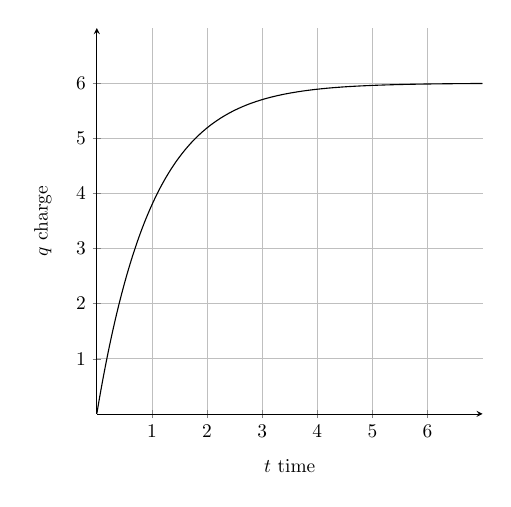
\begin{tikzpicture}[scale=0.7]
			\begin{axis}[
				x=1cm,y=1cm,
				axis lines=middle,
				ymajorgrids=true,
				xmajorgrids=true,
				xmin=0,
				xmax=7,
				ymin=0,
				x label style={at={(axis description cs:0.5,-0.1)},anchor=north},
				y label style={at={(axis description cs:-0.1,0.5)},rotate=90,anchor=south},
				xlabel=$t$ time,
				ylabel=$q$ charge,
				ymax=7,
				xtick={0,1,...,6},
				ytick={0,1,...,6},]
			\end{axis}
			\draw[domain=0:7,samples=1000] plot ({\x},{(6*(1-(e^(-\x))))});
		\end{tikzpicture}
		
		
		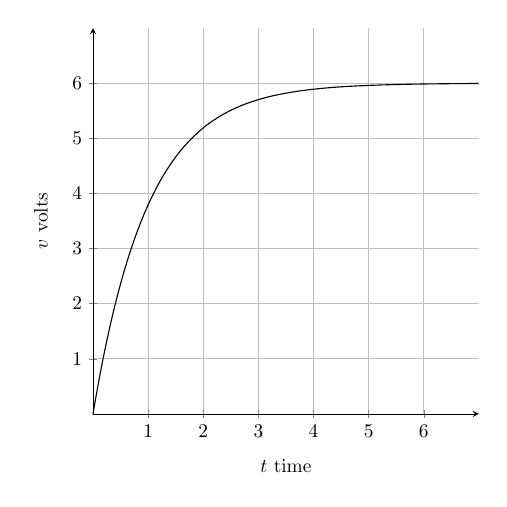
\begin{tikzpicture}[scale=0.7]
			\begin{axis}[
				x=1cm,y=1cm,
				axis lines=middle,
				ymajorgrids=true,
				xmajorgrids=true,
				xmin=0,
				xmax=7,
				ymin=0,
				x label style={at={(axis description cs:0.5,-0.1)},anchor=north},
				y label style={at={(axis description cs:-0.1,0.5)},rotate=90,anchor=south},
				xlabel=$t$ time,
				ylabel=$v$ volts,
				ymax=7,
				xtick={0,1,...,6},
				ytick={0,1,...,6},]
			\end{axis}
			\draw[domain=0:7,samples=1000] plot ({\x},{(6*(1-(e^(-\x))))});
		\end{tikzpicture}
		
		
		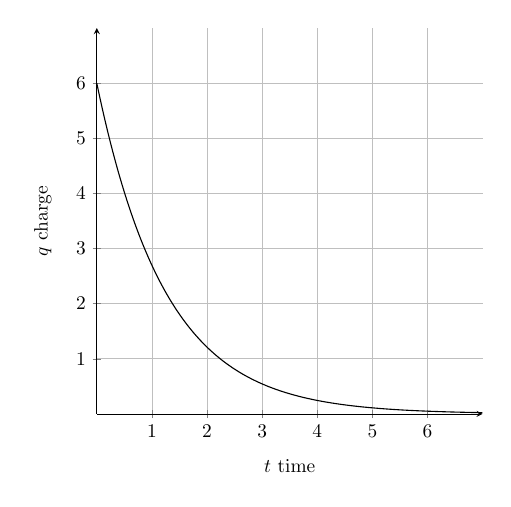
\begin{tikzpicture}[scale=0.7]
			\begin{axis}[
				x=1cm,y=1cm,
				axis lines=middle,
				ymajorgrids=true,
				xmajorgrids=true,
				xmin=0,
				xmax=7,
				ymin=0,
				x label style={at={(axis description cs:0.5,-0.1)},anchor=north},
				y label style={at={(axis description cs:-0.1,0.5)},rotate=90,anchor=south},
				xlabel=$t$ time,
				ylabel=$q$ charge,
				ymax=7,
				xtick={0,1,...,6},
				ytick={0,1,...,6},]
			\end{axis}
			\draw[domain=0:7,samples=1000] plot ({\x},{(6*(e^(-0.8*\x)))});
		\end{tikzpicture}
		
	\end{multicols}
	
	\section{Discharging graphs: }
	
	\begin{multicols}{3}
		{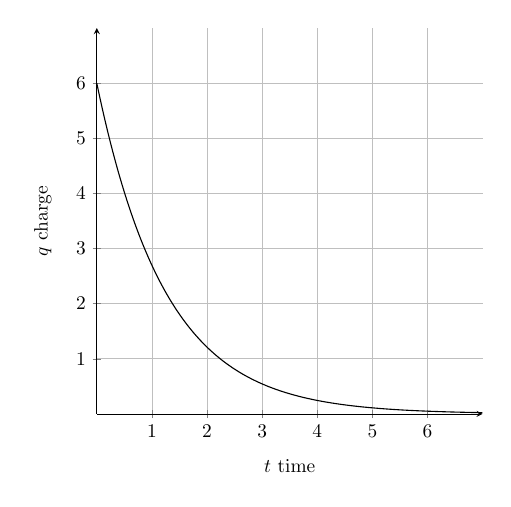
\begin{tikzpicture}[scale=0.7]
				\begin{axis}[
					x=1cm,y=1cm,
					axis lines=middle,
					ymajorgrids=true,
					xmajorgrids=true,
					xmin=0,
					xmax=7,
					ymin=0,
					x label style={at={(axis description cs:0.5,-0.1)},anchor=north},
					y label style={at={(axis description cs:-0.1,0.5)},rotate=90,anchor=south},
					xlabel=$t$ time,
					ylabel=$q$ charge,
					ymax=7,
					xtick={0,1,...,6},
					ytick={0,1,...,6},]
				\end{axis}
				\draw[domain=0:7,samples=1000] plot ({\x},{(6*(e^(-0.8*\x)))});
			\end{tikzpicture}
			
			\begin{center}
				\captionof*{figure}{\qquad \qquad Gradient: $\frac{\delta q}{\delta t} = I $}
		\end{center}}
		
		{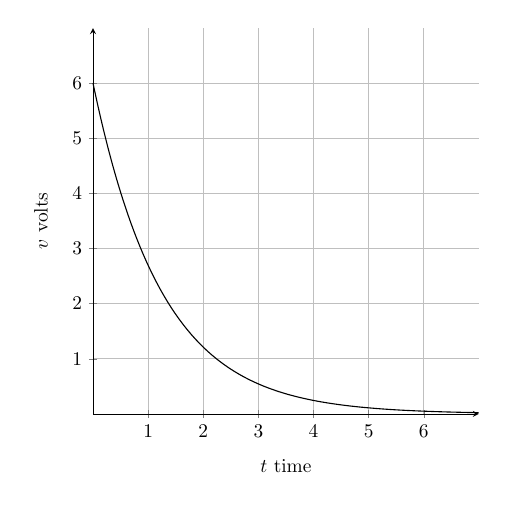
\begin{tikzpicture}[scale=0.7]
				\begin{axis}[
					x=1cm,y=1cm,
					axis lines=middle,
					ymajorgrids=true,
					xmajorgrids=true,
					xmin=0,
					xmax=7,
					ymin=0,
					x label style={at={(axis description cs:0.5,-0.1)},anchor=north},
					y label style={at={(axis description cs:-0.1,0.5)},rotate=90,anchor=south},
					xlabel=$t$ time,
					ylabel=$v$ volts,
					ymax=7,
					xtick={0,1,...,6},
					ytick={0,1,...,6},]
				\end{axis}
				\draw[domain=0:7,samples=1000] plot ({\x},{(6*(e^(-0.8*\x)))});
			\end{tikzpicture}
			\begin{center}
				\captionof*{figure}{\qquad \qquad Gradient: $\frac{\delta V}{\delta t}$}
		\end{center}}
		
		{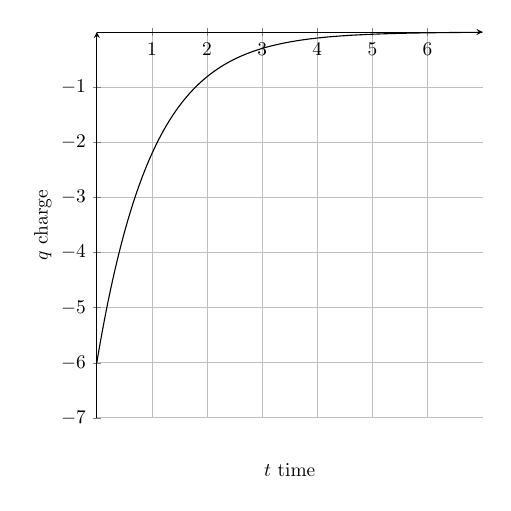
\begin{tikzpicture}[scale=0.7]
				\begin{axis}[
					x=1cm,y=1cm,
					axis lines=middle,
					ymajorgrids=true,
					xmajorgrids=true,
					xmin=0,
					xmax=7,
					ymin=-7,
					x label style={at={(axis description cs:0.5,-0.1)},anchor=north},
					y label style={at={(axis description cs:-0.1,0.5)},rotate=90,anchor=south},
					xlabel=$t$ time,
					ylabel=$q$ charge,
					ymax=0,
					xtick={0,1,...,6},
					ytick={0,-1,...,-7},]
				\end{axis}
				\draw[domain=0:7,samples=1000] plot ({\x},{1+(6*(1-(e^(-\x))))});
			\end{tikzpicture}
			\begin{center}
				\captionof*{figure}{\qquad \qquad Gradient: $\frac{\delta I}{\delta t}$}
		\end{center}}
	\end{multicols}
	
	\section{Dis/charging capacitor circuit: }
	\begin{center}
		{\begin{circuitikz} 
				\draw (0,0) to [short, *-] (0,-2)   to (8,-2)  to (8,-1)  to [short, *-, l^=B] (8,-1); 
				\draw (0,0) to (0,2) to [battery] (8,2) to (8,1) to [short, *-, l^=A] (8,1);
				\draw (0,0) to [capacitor] (4,0) to [vR] (7 ,0) to [short, *-] (8,0);
			\end{circuitikz}
			\captionof*{figure}{{\small A: Charging at 63\% every $\tau$.\\B: Discharging at 37\% every $\tau$}}}
	\end{center}

	\section{Dis/charging time formula: }
	\[\tau = RC\]
	$$\text{The convention is that after $5\tau$ seconds the capacitor discharges.} $$
\end{document}     